%                                                                 aa.dem
% AA vers. 9.1, LaTeX class for Astronomy & Astrophysics
% demonstration file
%                                                       (c) EDP Sciences
%-----------------------------------------------------------------------
%
%\documentclass[referee]{aa} % for a referee version
%\documentclass[onecolumn]{aa} % for a paper on 1 column  
%\documentclass[longauth]{aa} % for the long lists of affiliations 
%\documentclass[letter]{aa} % for the letters 
%\documentclass[bibyear]{aa} % if the references are not structured 
%                              according to the author-year natbib style

%
\documentclass{aa}  

%
\usepackage{graphicx}
%%%%%%%%%%%%%%%%%%%%%%%%%%%%%%%%%%%%%%%%
\usepackage{txfonts}
\usepackage[svgnames]{xcolor}
%%%%%%%%%%%%%%%%%%%%%%%%%%%%%%%%%%%%%%%%
% \usepackage[options]{hyperref}
% To add links in your PDF file, use the package "hyperref"
% with options according to your LaTeX or PDFLaTeX drivers.
%
\usepackage{hyperref}         % automagic cross-referencing
\usepackage{cleveref}
\renewcommand{\arraystretch}{1.3}
\newcommand\numberthis{\addtocounter{equation}{1}\tag{\theequation}}
% defines the color of hyperref objects
% Blending two colors:  blue!80!black  =  80% blue and 20% black
\hypersetup{ % this is just my personal choice, feel free to change things
    colorlinks,
    linkcolor={red!50!black},
    citecolor={blue!20!purple!80!black},
    urlcolor={blue!80!black},
    breaklinks=true}
\urlstyle{same}
\begin{document} 


   \title{A numerical study of the Cosmic Microwave Background}

   \subtitle{AST5220 - Cosmology II \colorbox{Plum}{maybe change title?}}

   \author{Candidate 15011
        %   \inst{1}
          }

   \institute{Institute of Theoretical Astrophysics (ITA), University of Oslo}

   \date{\today}

% \abstract{}{}{}{}{} 
% 5 {} token are mandatory
 
  \abstract

  {CONTEXT}
  {AIMS}
  {METHODS}
  {RESULTS}
  {CONCLUSIONS}\keywords{cosmic background radiation - large-scale structure of Universe}

   \maketitle
%
%-------------------------------------------------------------------
\section{Introduction}\label{sec: introduction}
\colorbox{Plum}{TODO: proper intro when finished} \\
% \colorbox{Plum}{does it make sense to have the links here?} 

In this work, I extensively reference the 2018 Planck results \citep[see][]{Planck}, which serve as the fiducial cosmology. The theoretical framework for this study, including derivations and discussions, is based on material from the AST5220 - Cosmology II course taught by Hans A. Winther at the University of Oslo \citep[see][]{Course}. All computational codes used in this work are available on my \href{https://github.com/paljettrosa/AST5220}{GitHub repository}, with major components based on templates developed by Winther. \colorbox{Plum}{okay to write this? link your GitHub?}
% The templates for  and these templates are available on his \href{https://github.com/HAWinther/AST5220-Cosmology}{GitHub account}. 

\section{Milestone I: Background Cosmology}\label{sec: milestone I}
The evolution of the universe is governed by the interplay between different energy components, including radiation, matter, and dark energy. Understanding how these components influence the expansion history is essential for predicting the large-scale structure of the Universe and the Cosmic Microwave Background (CMB) fluctuations. This milestone focuses on modeling the background evolution of the Universe using the Friedmann equations, which describe how the Hubble parameter $H$, and thus time and distance measures, evolve with redshift. 

I will implement a numerical framework that takes in cosmological parameters and computes such key background quantities, and use this to fit to measurements of supernova luminosity distances. By completing this milestone, I aim to establish a robust computational framework that will serve as a foundation for later stages of the project, where I will analyze perturbations and extract information about CMB anisotropies. \colorbox{Plum}{correct?}
% The results will then be used for constraining cosmological parameters using observational data. 

\subsection{Theoretical framework}\label{subsec: I theory}
\subsubsection{Evolution of the Universe and the Hubble parameter}
The expansion of the Universe is governed by General Relativity, with the large-scale dynamics described by the Friedmann-Lemaître-Robertson-Walker (FLRW) metric. Assuming a homogeneous and isotropic universe, the metric is given by
\begin{equation}
    ds^2 = -c^2 dt^2 + a^2(t) \left[ \frac{dr^2}{1 - k r^2} + r^2 d\theta^2 + r^2 \sin^2\theta d\phi^2 \right],
\end{equation}
where $a(t) = 1/(1+z)$ is the dimensionless scale factor, with $z$ being the cosmological redshift. The constant $k$ determines the curvature of the Universe ($k = 0$ for a flat universe, $k > 0$ for a closed universe, and $k < 0$ for an open universe). 

The evolution of $a(t)$ is governed by the Friedmann equation, which is derived from Einstein's field equations:
\begin{equation}
    H^2 = \frac{8\pi G}{3} \sum_{i}\rho_i - \frac{k c^2}{a^2} \simeq \frac{8\pi G}{3} \sum_{i}\rho_i,
\end{equation}
Here, $H = \dot{a}/a$ is the Hubble parameter, and $\rho_i$ denotes the total energy density of some component (photons, baryons, etc.). In the second equality I have used that we can treat the curvature as its own component that is included in the sum, with energy density
\begin{equation}
  \rho_k = -\frac{3}{8\pi G}\frac{k c^2}{a^2}. \label{eq:rho k}
\end{equation}
It is essential to know not only how the curvature ``energy density'' scales with $a$, but the other components as well. To understand this, we start with the continuity equation for a perfect fluid, which is a very accurate description of the energy density components in the Universe on the largest scales, applied to a homogeneous and isotropic universe:
\begin{equation}
  \frac{d\rho}{dt} + 3H (\rho_i+ p_i) = \frac{d\rho}{dt} + \frac{3}{a}\frac{da}{dt} \rho_i(1 + w_i) = 0.
\end{equation}
Here, $p_i$ is the pressure of the fluid, and $w_i=p_i/\rho_i$ is the equation of state parameter, which is constant for the fluids considered in conventional cosmology. This differential equation is easily solved by separating variables and integrating, which gives us:
\begin{equation}
  \rho_i(a) = \rho_{i0} a^{-3(1+w_i)},
\end{equation}
where $\rho_{i0}$ is the present-day density.

On universal scales, non-relativistic matter can essentially be treated as pressureless, hence $w_m = w_b=w_\text{CDM}=0$ and thus $\rho_m \propto a^{-3}$. This corresponds to the dilution of a density field in an expanding volume. Furthermore, neutrinos are so light that they can still be treated as relativistic (radiation), and we therefore have $w_r=w_\gamma=w_\nu=1/3$, which implies $\rho_r\propto a^{-4}$. Radiation is also diluted as the Universe expands, and the extra factor of $a^{-1}$ comes from redshifting of relativistic particles in an expanding universe. From eq. \eqref{eq:rho k} we indeed see that we can treat curvature as a perfect fluid with equation of state $w_k=-1/3$, while dark energy, represented by the cosmological constant $\Lambda$, remains constant in time, hence $w_\Lambda=-1$.

A much more convenient way of writing the Friedmann equation can be derived by defining the critical density, which is the density required for a flat universe ($k=0$):
\begin{equation}
  \rho_c = \frac{3 H^2}{8 \pi G}.
\end{equation}
We may then define the dimensionless density parameters, which describe how much of the total energy density each component $i$ contributes:
\begin{equation}
  \Omega_i = \frac{\rho_{i}}{\rho_c}.
\end{equation}
Substituting this into the Friedmann equation gives us then
\begin{equation}
  H^2 = \frac{8\pi G}{3} \sum_i \Omega_{i}\rho_c = H^2\sum_i \Omega_{i}, \label{eq:H squared}
\end{equation}
which shows us explicitly that the density parameters always must sum up to unity. We would like to rewrite this in terms of quantities that we can actually measure today, such as the present day density parameters $\Omega_{i0}$. In that case, $H^2$ becomes $H_0^2$ on the right-hand side of eq. \eqref{eq:H squared}. Furthermore, since we know how the density components scale with $a$, we may write
\begin{equation}
  H^2 = H_0^2\sum_i \Omega_{i0}a^{-3(1+w_i)}. \label{eq:H squared 2}
\end{equation} 
The equivalency of this expression with eq. \eqref{eq:H squared} tells us that
\begin{equation}
  \Omega_{i}(a) = \frac{\Omega_{i0}a^{-3(1+w_i)}}{H^2(a)/H_0^2}, \label{eq:density params}
\end{equation}
Additionally, taking the square root on both sides of eq. \eqref{eq:H squared 2} and writing out the terms explicitly, we have
\begin{equation}
    H = H_0 \sqrt{(\Omega_{b0} + \Omega_{\text{CDM}0}) a^{-3} + (\Omega_{\gamma 0} + \Omega_{\nu 0}) a^{-4} + \Omega_{k0} a^{-2} + \Omega_{\Lambda 0}}.
\end{equation}

Eventually, I will need to use data to determine all but the photon and neutrino density parameters, which we know are given by
\begin{align}
    \Omega_{\gamma0} &= g\frac{\pi^2}{30}\frac{\left(k_\text{B}T_{\text{CMB}0}\right)^4}{\hbar^3c^5}\frac{8\pi G}{3H_0^2},
    \\
    \Omega_{\nu0} &= \frac{7}{8}N_\text{eff}\left(\frac{4}{11}\right)^{1/3}\Omega_{\gamma0}.
\end{align}
Here, $g=g_\gamma=g_\nu=2$, since photons and neutrinos both have 2 internal polarization states, while $T_{\text{CMB}0}$ is the present day value of the CMB temperature, and $N_\text{eff}$ is the effective number of relativistic degrees of freedom. 
% Together with the baryon ($\Omega_{b0}$), cold dark matter ($\Omega_{\text{CDM}0}$) and curvature ($\Omega_{k0}$) density parameters, we then get the dark energy density parameter from
% \begin{equation}
%     \Omega_{\Lambda0} = 1 - \left(\Omega_{k0} + \Omega_{b0} + \Omega_{\text{CDM}0} + \Omega_{\gamma0} + \Omega_{\nu0} \right),
% \end{equation}
% since the density parameters must all sum to unity. 

When integrating from the very early universe, using the scale factor $a$ as the time parameter becomes numerically challenging, as it rapidly decreases to vanishingly small values. To address this, I will therefore adopt the logarithmic time coordinate
\begin{equation}
    x = \log a,
\end{equation}
instead, which implies that $x=0$ today and $x=-\infty$ at the Big Bang. Expressed in terms of $\Omega_{m0}=\Omega_{b0}+\Omega_{\text{CDM}0}$ and $\Omega_{r0}=\Omega_{\gamma0}+\Omega_{\nu0}$, we can equivalently write the Hubble parameter as
\begin{equation}
    H = H_0 \sqrt{\Omega_{m0} e^{-3x} + \Omega_{r0} e^{-4x} + \Omega_{k0} e^{-2x} + \Omega_{\Lambda 0}}.
\end{equation}

A commonly used rescaled version of the Hubble parameter is the conformal Hubble parameter:
\begin{equation}
    \mathcal{H} = aH = H_0 \sqrt{\Omega_{m0} e^{-x} + \Omega_{r0} e^{-2x} + \Omega_{k0} + \Omega_{\Lambda 0}e^{2x}}. \label{eq:Hp}
\end{equation}
This naturally appears when rewriting cosmological equations in terms of the conformal time $\eta$, which I will present below. I will focus more on this version of the Hubble parameter, and it will become useful to know its first and second derivatives with respect to $x$, specifically in order to verify the validity of approximations I will make later on. After some tedious calculation, we find that these are
\begin{align*}
    \frac{d\mathcal{H}}{dx} &= \frac{H_0}{2}
    \frac{-\Omega_{m0}e^{-x} - 2\Omega_{r0}e^{-2x} + 2\Omega_{\Lambda0}e^{2x}}
    {\sqrt{\Omega_{m0}e^{-x} 
    + \Omega_{r0}e^{-2x}
    + \Omega_{k0} + \Omega_{\Lambda0}e^{2x}}},
    \\
    &= -\frac{H_0^2}{2\mathcal{H}}\left(\Omega_{m0}e^{-x} + 2\Omega_{r0}e^{-2x} - 2\Omega_{\Lambda0}e^{2x}\right), \numberthis \label{eq:dHpdx}
    \\
    \frac{d^2\mathcal{H}}{dx^2} &= \frac{H_0}{2}
    \left(\frac{\Omega_{m0}e^{-x} + 4\Omega_{r0}e^{-2x} + 4\Omega_{\Lambda0}e^{2x}}{\sqrt{\Omega_{m0}e^{-x} + \Omega_{r0}e^{-2x} + \Omega_{k0} + \Omega_{\Lambda0}e^{2x}}}\right.
    \\
    &\hspace{38pt}
    \left.- \frac{1}{2}\frac{\left(\Omega_{m0}e^{-x} + 2\Omega_{r0}e^{-2x} - 2\Omega_{\Lambda0}e^{2x}\right)^2}{\left(\Omega_{m0}e^{-x} + \Omega_{r0}e^{-2x} + \Omega_{k0} + \Omega_{\Lambda0}e^{2x}\right)^{3/2}}\right),
    \\
    &= \frac{H_0^2}{\mathcal{H}}\left[\frac{1}{2}\Omega_{m0}e^{-x} + 2\Omega_{r0}e^{-2x} + 2\Omega_{\Lambda0}e^{2x}- \frac{1}{H_0^2}\left(\frac{d\mathcal{H}}{dx}\right)^2\right]. \numberthis \label{eq:ddHpddx}
  \end{align*}


\subsubsection{Conformal time and distance measures}
The cosmic time $t$ is related to our time variable $x$ through
\begin{equation}
  \frac{dt}{dx} = \frac{dt}{da}\frac{da}{dx} = \frac{a}{\dot{a}} = \frac{1}{H},
\end{equation}
hence, to compute the cosmic time $t$ given our time coordinate $x$, we simply integrate this to get 
\begin{equation}
  t(x) = \int_{-\infty}^{x} \frac{dx'}{H(x')}.
\end{equation}
Evaluating this at $x=0$ (today), we obtain the age of the Universe.

While it will be interesting to solve our system of equations for $t$, it will be more useful to introduce the conformal time $\eta$. This is defined as
\begin{equation}
d\eta = \frac{cdt}{a} \hspace{5pt}\Leftrightarrow\hspace{5pt}\frac{d\eta}{dx} = \frac{c}{\mathcal{H}},
\end{equation}
and thus has units of length. The equation on the right can easily be numerically integrated to obtain $\eta(x)$, which describes how far light has traveled since the Big Bang. In other words, the comoving distance a photon has traveled since the start of the Universe is given by:
\begin{equation}
\chi = \eta_0 - \eta,
\end{equation}
where $\eta_0$ is the conformal time today. This quantity is also called the particle horizon, and it is a crucial concept in cosmology, as it represents the maximum comoving distance that light has traveled since the beginning of the Universe, thus determining its causal structure. 

The horizon is fundamental in defining distance measures in cosmology. We know that photons travel along null geodesics $ds^2 = 0$, and from the conformal time and the FLRW line element we see that this implies that the coordinate distance $r$ satisfies
\begin{equation}
  c dt = \frac{adr}{\sqrt{1 - k r^2}},
\end{equation}
for a radially traveling photon ($d\theta = d\phi = 0$). Changing the time coordinate to conformal time, we rewrite this as
\begin{equation}
  d\eta = \frac{dr}{\sqrt{1 - k r^2}},
\end{equation}
and integrating from emission at time $\eta$ to today ($\eta_0$), we get the comoving distance:
\begin{equation}
  \chi = \int_{\eta}^{\eta_0}  d\eta' = \int_{0}^{r} \frac{dr'}{\sqrt{1 - k r'^2}}.
\end{equation}
Solving this integral for different values of the curvature constant $k$, we obtain
\begin{equation}
  r = 
  \chi\begin{cases}
  \cfrac{\sin\left(\sqrt{|\Omega_{k0}|} H_0 \chi / c\right)}{\left(\sqrt{|\Omega_{k0}|} H_0 \chi / c\right)}, & \Omega_{k0} < 0 \quad \text{(Closed)}, \\
1, & \Omega_{k0} = 0 \quad \text{(Flat)}, \\
\cfrac{\sinh\left(\sqrt{|\Omega_{k0}|} H_0 \chi / c\right)}{\left(\sqrt{|\Omega_{k0}|} H_0 \chi / c\right)}, & \Omega_{k0} > 0 \quad \text{(Open)}.
\end{cases}
\end{equation}
This defines the proper radial coordinate $r$, which is used in all cosmological distance measures. 

The angular diameter distance relates an object's physical extent $D$ to its observed angular extent $\theta$ on the sky:
\begin{equation}
d_A = \frac{D}{\theta}.
\end{equation}
From the metric, we see that the transverse separation of a source at $r$ subtending an angle $d\theta$ is
\begin{equation}
  dD = a r d\theta,
\end{equation}
hence the angular diameter distance:
\begin{equation}
  d_A = a r,
\end{equation}
which simplifies to:
\begin{equation}
  d_A = a \chi,
\end{equation}
for a flat universe.

Even more relevant for this milestone is the luminosity distance, which is dependent on the measured brightness of standard candles like Type Ia supernovae. We know that the flux $F$ from a source with luminosity $L$ follows an inverse-square law:
\begin{equation}
  F = \frac{L}{4\pi d_L^2}.
\end{equation}
In an expanding universe, photons are redshifted and their arrival rate is also affected, leading to the relation:
\begin{equation}
  d_L = d_A (1 + z)^2 = \frac{d_A}{a^2}.
\end{equation}
This quantity is crucial in observational cosmology as it accounts for both the geometric distance and the redshifted energy of photons. It is therefore fundamental for interpreting supernovae observations and measuring cosmic expansion.



\subsubsection{Key cosmological epochs}
Though it also has been verified by numerous observations, based on the expression for the Hubble parameter it is not hard to see that the Universe must have gone through phases where its energy budget was (or will be) dominated by radiation, matter and dark energy, separately, in that order. This implies that there must have been a point in time where the Universe was equal amounts of radiation and matter (matter and dark energy), if we neglect the curvature and dark energy (radiation). At radiation-matter equality ($rm$) we have
\begin{equation}
    \Omega_{r,rm} = \Omega_{m,rm} 
    \hspace{5pt}\Leftrightarrow\hspace{5pt} 
    \Omega_{r0}e^{-4x_{rm}} = \Omega_{m0}e^{-3x_{rm}}, 
\end{equation}
and thus
\begin{equation}
  x_{rm} = \log\left(\frac{\Omega_{r0}}{\Omega_{m0}}\right).
\end{equation}
Using that $x = \log a$ and $z = 1/a - 1$ this gives us an expression for the redshift at $rm$:
\begin{equation}
  z_{rm} = \frac{\Omega_{m0}}{\Omega_{r0}} - 1.
\end{equation} 
Similarly, at matter-dark energy equality ($m\Lambda$) we have
\begin{equation}
  \Omega_{m0}e^{-3x_{m\Lambda}} = \Omega_{\Lambda0}
  \hspace{5pt}\Leftrightarrow\hspace{5pt}
  x_{m\Lambda} = \frac{1}{3}\log\left(\frac{\Omega_{m0}}{\Omega_{\Lambda0}}\right),
\end{equation}
and thus
\begin{equation}
  z_{m\Lambda} = \left(\frac{\Omega_{\Lambda0}}{\Omega_{m0}}\right)^{1/3} - 1.
\end{equation}

To ensure that the numerical results presented in this work agree with analytical expectations, it will be beneficial to have approximate expressions for the cosmic and conformal times in the different regimes. For a universe dominated by a single component with equation of state $w_i$ the cosmic time $t$ is given by
\begin{equation}
  t = \int_0^t dt' = \int_{-\infty}^{x}\frac{dx'}{H_0\sqrt{\Omega_{i0}e^{-3(1+w_i)x'}}}.
\end{equation}
When the Universe transitions between an era where its energy density is dominated by some component $\rho_j$ to some other component $\rho_i$, we may neglect all other components and compute an approximate expression for the cosmic time as function of $x$ by writing
\begin{equation}
  t_i(x) \approx t_{j,i} + \int_{x_{j,i}}^{x}\frac{dx'}{H_0\sqrt{\Omega_{i0}e^{-3(1+w_i)x'}}},
\end{equation}
where $x_{j,i}$ and $t_{j,i}$ correspond to their values when $\rho_j=\rho_i$. For radiation we simply have $x_{j,i}=-\infty$ and thus $t_{j,i}=0$, since the very early Universe was filled with relativistic particles, hence
\begin{equation}
  t_r(x) = \int_{{-\infty}}^{x}\frac{dx'}{H_0\sqrt{\Omega_{r0}e^{-4x'}}} = \frac{1}{2H_0\sqrt{\Omega_{r0}e^{-4x}}}.
\end{equation}
We see that radiation-matter equality occurs at
\begin{equation}
  t_{rm} = t_r(x_{rm}) = \frac{\Omega_{r0}^{3/2}}{2H_0\Omega_{m0}^2},
\end{equation}
and for matter it then follows
\begin{align*}
  t_m(x) &\approx t_{rm} + \int_{x_{rm}}^{x}\frac{dx'}{H_0\sqrt{\Omega_{m0}e^{-3x'}}}, 
  \\
  &= \frac{\Omega_{r0}^{3/2}}{2H_0\Omega_{m0}^2}+\frac{2}{3H_0}\left[\frac{1}{\sqrt{\Omega_{m0}e^{-3x}}} - \frac{\Omega_{r0}^{3/2}}{H_0\Omega_{m0}^2} \right],
  \\
  &= \frac{1}{3H_0}\left[\frac{2}{\sqrt{\Omega_{m0}e^{-3x}}} - \frac{\Omega_{r0}^{3/2}}{2\Omega^2_{m0}} \right], \numberthis
\end{align*}
with matter-dark energy equality occuring at
\begin{equation}
  t_{m\Lambda} = \frac{1}{3H_0}\left[\frac{2}{\sqrt{\Omega_{\Lambda0}}} - \frac{\Omega_{r0}^{3/2}}{2\Omega^2_{m0}} \right].
\end{equation}
Lastly, for dark energy we have
\begin{align*}
  t_\Lambda(x) &\approx t_{m\Lambda} + \int_{x_{m\Lambda}}^{x}\frac{dx'}{H_0\sqrt{\Omega_{\Lambda0}}}, 
  \\
  &= \frac{1}{3H_0}\left[\frac{2}{\sqrt{\Omega_{\Lambda0}}} - \frac{\Omega_{r0}^{3/2}}{2\Omega^2_{m0}} \right] + \frac{1}{H_0\sqrt{\Omega_{\Lambda0}}}\left[x - \frac{1}{3}\log\left(\frac{\Omega_{m0}}{\Omega_{\Lambda0}}\right)\right],
  \\
  &= \frac{1}{H_0\sqrt{\Omega_{\Lambda0}}}\left[x+\frac{2}{3}-\frac{1}{3}\log\left(\frac{\Omega_{m0}}{\Omega_{\Lambda0}}\right)-\frac{\sqrt{\Omega_{\Lambda0}}\Omega_{r0}^{3/2}}{6\Omega^2_{m0}}\right]. \numberthis
\end{align*}
From these derived expressions, it is obvious that $a\propto t^{1/2}$ in the radiation dominated era, $a\propto t^{2/3}$ in the matter era and $a\propto e^{H_0\sqrt{\Omega_{\Lambda0}}t}$ in the dark energy era, which is the expected result.

Following an analogous approach for the conformal time, it is straight-forward to show that since
\begin{equation}
  \eta_i(x) \approx \eta_{j,i} + \int_{x_{j,i}}^{x}\frac{cdx'}{H_0\sqrt{\Omega_{i0}e^{-(1+3w_i)x'}}},
\end{equation}
we have the following approximate expressions:
\begin{align}
  \eta_r(x) &= \frac{c}{H_0\sqrt{\Omega_{r0}e^{-2x}}},
  \\
  \eta_m(x) &= \frac{c}{H_0}\left[\frac{2}{\sqrt{\Omega_{m0}e^{-x}}} - \frac{\sqrt{\Omega_{r0}}}{\Omega_{m0}} \right],
  \\
  \eta_\Lambda(x) &= -\frac{c}{H_0}\left[\frac{1}{\sqrt{\Omega_{\Lambda0}e^{2x}}} +\frac{\sqrt{\Omega_{r0}}}{\Omega_{m0}} - \frac{3}{\Omega_{m0}^{1/3}\Omega_{\Lambda0}^{1/6}} \right],
\end{align}
with the conformal equality times:
\begin{align}
  \eta_{rm} &= \frac{c}{H_0}\frac{\sqrt{\Omega_{r0}}}{\Omega_{m0}},
  \\
  \eta_{m\Lambda} &= \frac{c}{H_0}\left[\frac{2}{\Omega_{m0}^{1/3}\Omega_{\Lambda0}^{1/6}} - \frac{\sqrt{\Omega_{r0}}}{\Omega_{m0}}\right].
\end{align}

To be able to actually test the validity of the approximations made above, it is essential to use them to compute the expected values of some scaled expressions, as this will make it easier to see the relative errors. Obviously, in an era dominated by component $i$ we have
\begin{equation}
    \mathcal{H}_i \approx H_0\sqrt{\Omega_{i0}e^{-(1+3w_i)}},
\end{equation}
and in the radiation dominated era we thus have
\begin{align}
  \left(\frac{d\mathcal{H}}{dx}\right)_r &= -H_0\sqrt{\Omega_{r0}}e^{-x}=-\mathcal{H}_r 
  \hspace{5pt}\Leftrightarrow\hspace{9pt}\left(\frac{1}{\mathcal{H}}\frac{d\mathcal{H}}{dx}\right)_r=-1,
  \\
  \left(\frac{d^2\mathcal{H}}{dx^2}\right)_r &= H_0\sqrt{\Omega_{r0}}e^{-x}=\mathcal{H}_r
  \hspace{18pt}\Leftrightarrow\hspace{5pt}\left(\frac{1}{\mathcal{H}}\frac{d^2\mathcal{H}}{dx^2}\right)_r=1.
\end{align}
Similarly, we have
\begin{align}
  \left(\frac{d\mathcal{H}}{dx}\right)_m &= -\frac{\mathcal{H}_m}{2} 
  \hspace{5pt}\Leftrightarrow\hspace{10pt}\left(\frac{1}{\mathcal{H}}\frac{d\mathcal{H}}{dx}\right)_m=-\frac{1}{2},
  \\
  \left(\frac{d^2\mathcal{H}}{dx^2}\right)_m &= \frac{\mathcal{H}_m}{4}
  \hspace{12pt}\Leftrightarrow\hspace{5pt}\left(\frac{1}{\mathcal{H}}\frac{d^2\mathcal{H}}{dx^2}\right)_m=\frac{1}{4}.
\end{align}
in the matter dominated era, and
\begin{equation}
  \mathcal{H}_\Lambda = \left(\frac{d\mathcal{H}}{dx}\right)_\Lambda = \left(\frac{d^2\mathcal{H}}{dx^2}\right)_\Lambda = H_0\sqrt{\Omega_{\Lambda0}}e^{x},
\end{equation}
in the dark energy dominated era. From the latter it is obvious that
\begin{equation}
  \left(\frac{1}{\mathcal{H}}\frac{d\mathcal{H}}{dx}\right)_\Lambda = \left(\frac{1}{\mathcal{H}}\frac{d^2\mathcal{H}}{dx^2}\right)_\Lambda = 1.
\end{equation} 


\subsubsection{Onset of acceleration}
Later on, when we will analyze the observed CMB power spectrum, it will be interesting to know when the expansion of the Universe started to accelerate. It is a well known fact that the expansion rate (governed by $\dot{a}$) is increasing as of today, and that we are in the early stage of a dark energy dominated era. We have the second Friedmann equation
\begin{equation}
    \frac{\ddot{a}}{a} = -\frac{4\pi G}{3}\sum_i \rho_i\left(1 + 3w_i \right),
\end{equation}
where the sum runs over all components (matter, radiation, etc.). The onset of acceleration occurs when $\ddot{a}$ switches sign, i.e., when
\begin{equation}
    \sum_i \rho_i\left(1 + 3w_i \right) = 0.
\end{equation}
Assuming that this happens well after the radiation dominated era, we can approximate this as
\begin{equation}
  \rho_m(x_\text{acc})- 2\rho_\Lambda(x_\text{acc}) = 0 \label{eq: equal acc time}
\end{equation}
Using that the expression \eqref{eq:density params} for the density parameters at arbitrary $a$, we can rewrite eq. \eqref{eq: equal acc time} to get
\begin{equation}
  \Omega_{m0}e^{-3x_\text{acc}} = 2\Omega_{\Lambda0}
  \hspace{5pt}\Leftrightarrow\hspace{5pt}
  x_\text{acc} = \frac{1}{3}\log\left(\frac{\Omega_{m0}}{2\Omega_{\Lambda0}}\right).
\end{equation}
This corresponds to a redshift
\begin{equation}
  z_\text{acc} = \left(\frac{2\Omega_{\Lambda0}}{\Omega_{m0}}\right)^{1/3}-1.
\end{equation}
Obviously, $t_\text{acc}<t_{m\Lambda}$, so we can make the same approximation this time, hence
% \begin{equation}
%   t_\text{acc} = t_{rm} + \int^{x_\text{acc}}_{x_{rm}}\frac{dx}{H_0\sqrt{\Omega_{m0}e^{-3x}}} = \frac{1}{3H_0}\left(\sqrt{\frac{2}{\Omega_{\Lambda0}}} -\frac{\Omega_{r0}^{3/2}}{2\Omega_{m0}^2}\right).
% \end{equation}
\begin{equation}
    t_\text{acc} = t_m(x_\text{acc}) = \frac{1}{3H_0}\left[\sqrt{\frac{2}{\Omega_{\Lambda0}}} -\frac{\Omega_{r0}^{3/2}}{2\Omega_{m0}^2}\right],
\end{equation}
with the conformal time being
\begin{equation}
    \eta_\text{acc} = \eta_m(x_\text{acc}) = \frac{c}{H_0}\left[\frac{2^{5/6}}{\Omega_{m0}^{1/3}\Omega_{\Lambda0}^{1/6}} - \frac{\sqrt{\Omega_{r0}}}{\Omega_{m0}}\right].
\end{equation}


\subsubsection{The Universe today}
It is of course a great consistency check to see if I am able to replicate the values for the age of the Universe and its horizon size today, and we can use the expressions derived above to do so. Following the approximations I have done up until this point, we have
\begin{align}
  t_0 &\approx t_{\Lambda}(0) = \frac{1}{H_0\sqrt{\Omega_{\Lambda0}}}\left[\frac{2}{3}-\frac{1}{3}\log\left(\frac{\Omega_{m0}}{\Omega_{\Lambda0}}\right)-\frac{\sqrt{\Omega_{\Lambda0}}\Omega_{r0}^{3/2}}{6\Omega^2_{m0}}\right],
  \\
  \eta_0 &\approx \eta_\Lambda(0) = -\frac{c}{H_0}\left[\frac{1}{\sqrt{\Omega_{\Lambda0}}} +\frac{\sqrt{\Omega_{r0}}}{\Omega_{m0}} - \frac{3}{\Omega_{m0}^{1/3}\Omega_{\Lambda0}^{1/6}} \right].
\end{align}
as we know that we currently are in the beginning of a dark energy dominated era.
% \colorbox{Plum}{should I just remove and present values in results? redundant here?}


\subsubsection{Initial conditions}
To numerically solve for conformal time $\eta$ and cosmic time $t$, we need appropriate initial conditions. Integrating from $x = -\infty$ (i.e., the Big Bang) is of course impossible, and we may therefore choose an early starting time $x_{\text{start}}$ instead, and use the analytical approximations in the radiation-dominated era:
\begin{align}
  \eta(x_{\text{start}}) &= \frac{c}{H\sqrt{\Omega_{r0}e^{-2x_\text{start}}}} \approx \frac{c}{H(x_{\text{start}})},
  \\
  t(x_{\text{start}}) &= \frac{1}{2H\sqrt{\Omega_{r0}e^{-4x_\text{start}}}} \approx \frac{1}{2H(x_{\text{start}})}.
\end{align}
This ensures a smooth transition between analytical and numerical solutions, minimizing errors when solving for the full evolution of $\eta(x)$ and $t(x)$.

\colorbox{Plum}{should this section be somewhere else?}


\subsubsection{The \texorpdfstring{$\chi^2$}{Lg}-method}
After having established the theoretical framework describing the evolution of the Universe, we now turn to how observational data can be used to constrain cosmological parameters. One of the most powerful tools for this is the study of Type Ia supernovae, which serve as standard candles for measuring the expansion history of the Universe. Given their intrinsic luminosity, the observed flux allows us to determine their luminosity distance $d_L$ as a function of redshift $z$, providing a direct probe of the Universe's geometry and expansion.

To quantitatively compare theoretical models to observational data, we define the so-called chi-squared statistic:
\begin{equation}
  \chi^2(h, \Omega_{m0}, \Omega_{k0}) = \sum_{i=1}^{N} \frac{ \left[ d_L(z_i, h, \Omega_{m0}, \Omega_{k0}) - d_L^{\text{obs}}(z_i) \right]^2 }{\sigma_i^2},
\end{equation}
where $N$ is the number of data points, $d_L^{\text{obs}}(z_i)$ represents the measured luminosity distance at redshift $z_i$, and $\sigma_i$ is the associated measurement uncertainty. This function quantifies how well a given set of parameters $(h, \Omega_{m0}, \Omega_{k0})$ fits the data: a lower $\chi^2$ value corresponds to a better fit. 


\subsection{Implementation details}\label{subsec: I methods}
\subsubsection{The fiducial model}
As mentioned in section \ref{sec: introduction}, I will adopt the best-fit Planck 2018 cosmology \citep[see][]{Planck} as my fiducial model, which includes the following parameters:
\begin{align*}
    h &= 0.67,
    \\
    T_{\text{CMB}0} &= 2.7255\,\text{K},
    \\
    N_\text{eff} &= 3.046,
    \\
    \Omega_{b0} &= 0.05,
    \\
    \Omega_{\text{CDM}0} &= 0.267,
    \\
    \Omega_{k0} &= 0.
\end{align*}
Here, $h$ is the dimensionless Hubble constant, which is related to the commonly presented Hubble constant through
\begin{equation*}
    H_0 = 100h\,\text{km\,s}^{-1}\text{\,Mpc}^{-1}.
\end{equation*}
The photon and neutrino density parameters are easily calculated using the values for $T_{\text{CMB}0}$ and $N_\text{eff}$, and since all the density parameters must sum up to unity, we have
\begin{align*}
  \Omega_{\gamma0} &= 5.50896\times10^{-5},
  \\
  \Omega_{\nu0} &=  3.81093\times10^{-5},
  \\
  \Omega_{\Lambda0} &= 0.682907.
\end{align*}

\subsubsection{Main program structure}
As mentioned in section \ref{sec: introduction}, all the code I use is located on my \href{https://github.com/paljettrosa/AST5220}{GitHub account}. In this section I will specify which files are relevant for this milestone, and roughly what they contain and how they should be implemented. All of the source codes, which are implemented in C++, are located in the \verb|src| folder, including the main program \verb|Main.cpp|. Naturally, the \verb|scripts| folder contains Python scripts, wherein NumPy and Matplotlib have been used for plotting and analyzing the results. The \verb|data| and \verb|results| folders contain data and outputs from the source code, respectively, in the form of \verb|.txt| files, while figures are placed in \verb|figs|. The \verb|Makefile| and \verb|README.md| are not contained within any folder, and are completely written by Winther. \colorbox{Plum}{should I remove stuff about folders?}

The evolution of the conformal and cosmic times, Hubble parameter, density parameters and related quantities are computed using the \verb|BackgroundCosmology| class, implemented in \verb|BackgroundCosmology.cpp| and \verb|BackgroundCosmology.h|. Necessary constants and units are defined in their SI-unit values in \verb|Utils.h|, as well as some convenient data types. The fundamental equations governing the expansion are integrated numerically using a GSL-based ODE solver (see \verb|ODESolver.cpp| and \verb|ODESolver.h|). The solutions for $t(x)$ and $\eta(x)$ are stored at discrete values of $x$ and are interpolated using cubic splines (see \verb|Spline.cpp| and \verb|Spline.h|) for efficient lookup, which also ensure smooth evaluations of these quantities at any redshift. This is implemented within the \verb|BackgroundCosmology| class, and all results produced here are written to file and analyzed in \verb|time_evolution.py|. \colorbox{Plum}{should C++, Python, GNU, etc. be cited?}


\subsubsection{Integration limits and points}
When integrating to solve for $\eta$ and $t$, I chose to use $x_\text{min}=-21.0$ and $x_\text{max}=6.0$ as integration limits, with $n=1\,000$ points. However, when splining the results I used $x_\text{min}=-20.0$ and $x_\text{max}=5.0$ instead, so as to not include the likely more unstable endpoints, and with $n=100(x_\text{max}-x_\text{min})+1=2501$ points for smoother visualization.


\subsubsection{Supernova fitting}
To constrain cosmological parameters ($h, \Omega_{m0}, \Omega_{k0}$), I performed a Markov Chain Monte Carlo (MCMC) fit to Type Ia supernova data (see \verb|supernovadata.txt|), which is implemented in \verb|SupernovaFitting.h|. The MCMC chain consists of 10$\,$000 samples, where I have treated the 200 first samples are as burn-in time and thus discarded them. The results are further analyzed in \verb|supernova.py|, where I visualize the accepted samples within the $(\chi^2-\chi^2_\text{min})<1\sigma$ and $(\chi^2-\chi^2_\text{min})<2\sigma$, constraints in the $(\Omega_{m0},\Omega_{\Lambda0})$-plane, corresponding to 68.3\% and 95.45\% confidence levels, repsectively. I have used tabulated values of $1\sigma=3.53$ and $2\sigma=8.02$ \citep[see][]{Chi2}, since we have $k=3$ degrees of freedom. This is because we really have four parameters $(h, \Omega_{m0}, \Omega_{k0}, \Omega_{\Lambda0})$, but the constraint that all the density parameters must sum up to unity, which eliminates one d.o.f. 


\subsection{Results and discussions}\label{subsec: I results}
\subsubsection{Test of numerical stability}
\begin{figure}
    \centering
    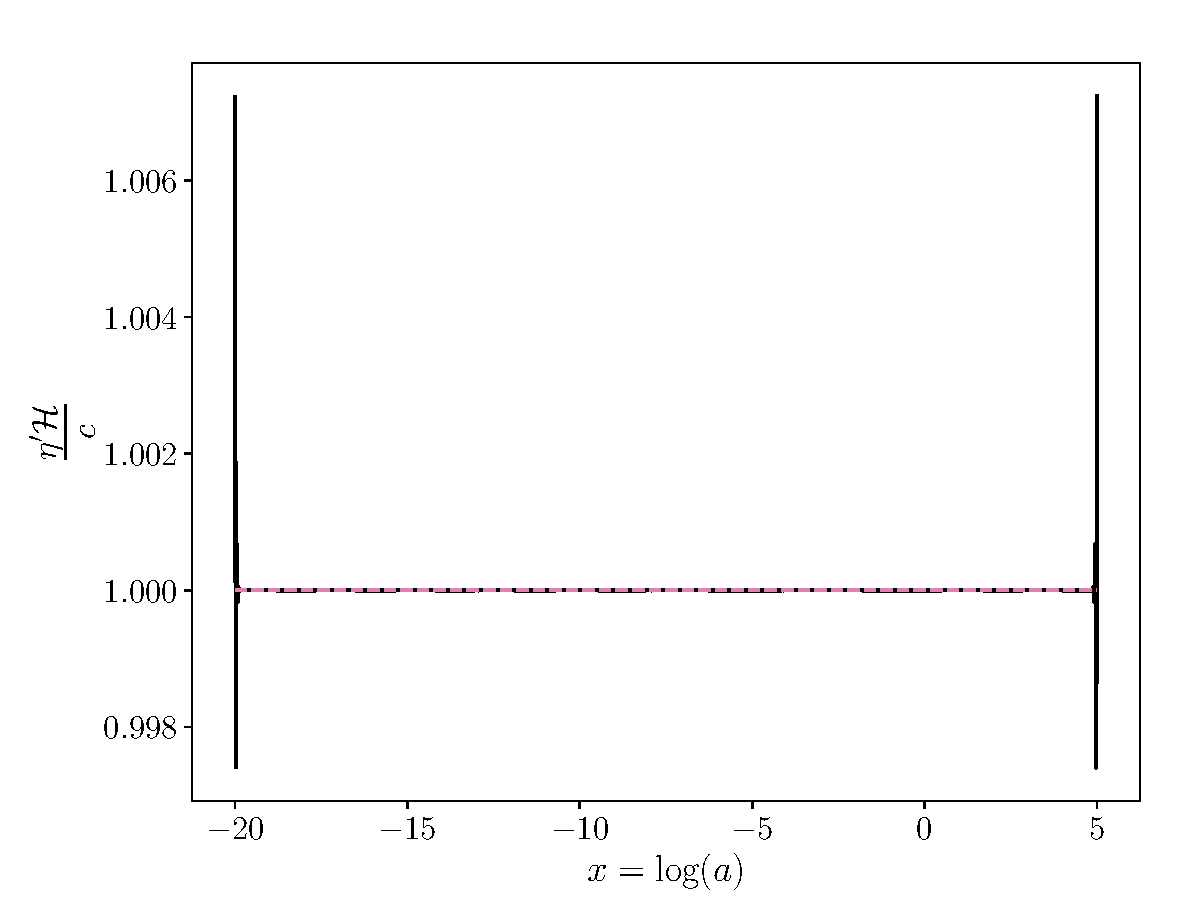
\includegraphics[width=\columnwidth]{/Users/paljettrosa/Documents/GitHub/AST5220/figs/numerical_stability.pdf}
    \caption{Comparison of the numerically computed conformal time derivative  $\eta'\mathcal{H}/c$ with the expected value of 1 (pink line). The small deviations on the order of $\lesssim 10^{-5}$ confirm the numerical stability of the integration.}\label{fig:numerical stability}
\end{figure}

\colorbox{Plum}{should this section come later?}

To ensure that the numerical solutions are stable, I have plotted $\eta'\mathcal{H}/c$ as function of $x$ in figure \ref{fig:numerical stability}, since this quantity should remain close to unity throughout the range. The scatter points, which were obtained by taking the derivative of the spline for $\eta$, show small deviations from 1, on the order of $\lesssim 10^{-5}$, indicating that the numerical error is very small. It also remains bounded bounded throughout the range of $x$, suggesting that the ODE solver maintains stability and does not accumulate significant numerical drift. The slight periodic variations could result from finite step sizes in the integration, or have something to do with interpolation errors between the integration points, but they are well within an acceptable tolerance. \colorbox{Plum}{is this a reasonable argument?}


\subsubsection{The conformal Hubble parameter}
\begin{figure}
  \centering
  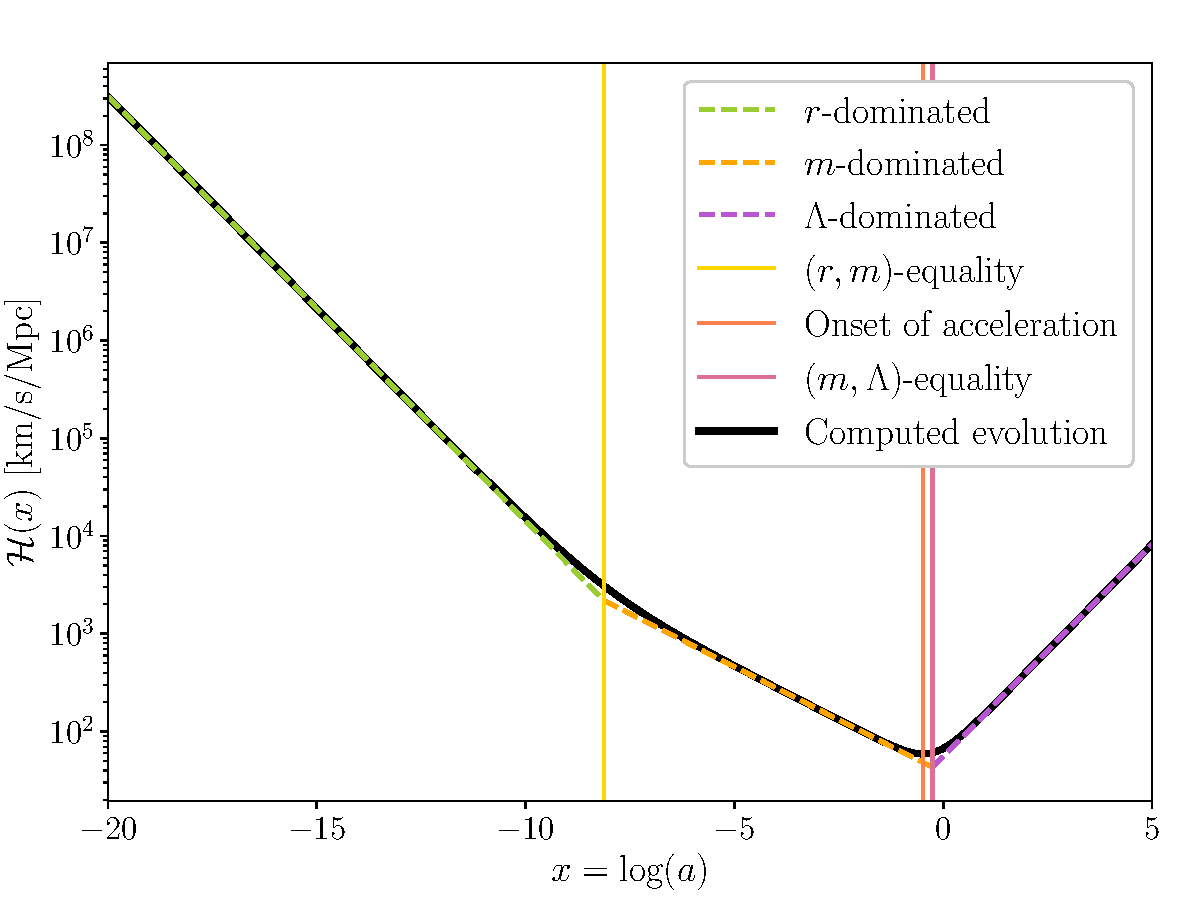
\includegraphics[width=\columnwidth]{/Users/paljettrosa/Documents/GitHub/AST5220/figs/H_prime.pdf}
  \caption{Exact evolution of the conformal Hubble parameter $\mathcal{H}(x)$ (black) compared with approximations (dashed). The onset of acceleration is visible as a departure from matter-like scaling, occuring at the trough of the exact solution. \colorbox{Plum}{okay to write this here instead of main text?}}\label{fig:H_prime}
\end{figure}


In figure \ref{fig:H_prime} I have plotted the exact evolution of the conformal Hubble parameter $\mathcal{H}(x)$ (black solid line), with approximations in the different cosmological epochs overplotted (dashed lines). Green, orange and purple correspond to radiation-, matter- and dark energy-dominated eras, respectively, with the yellow, red and pink vertical lines marking radiation-matter equality, onset of acceleration, and matter-dark energy equality. We see that the approximations closely follow the exact solution, staying at the correct order of magnitude at all times, although the deviations are significant close to the equality times. These are of course to be expected, since the approximations were derived under the assumption of the Universe only containing the dominating component within the different eras, which of course is not realistic as we transition from one to another. Thus, the result is still a great validation for the approximations, which indicates that we can safely use them to verify the numerical solutions for $\eta$ and $t$.

\begin{figure*}
    \centering
    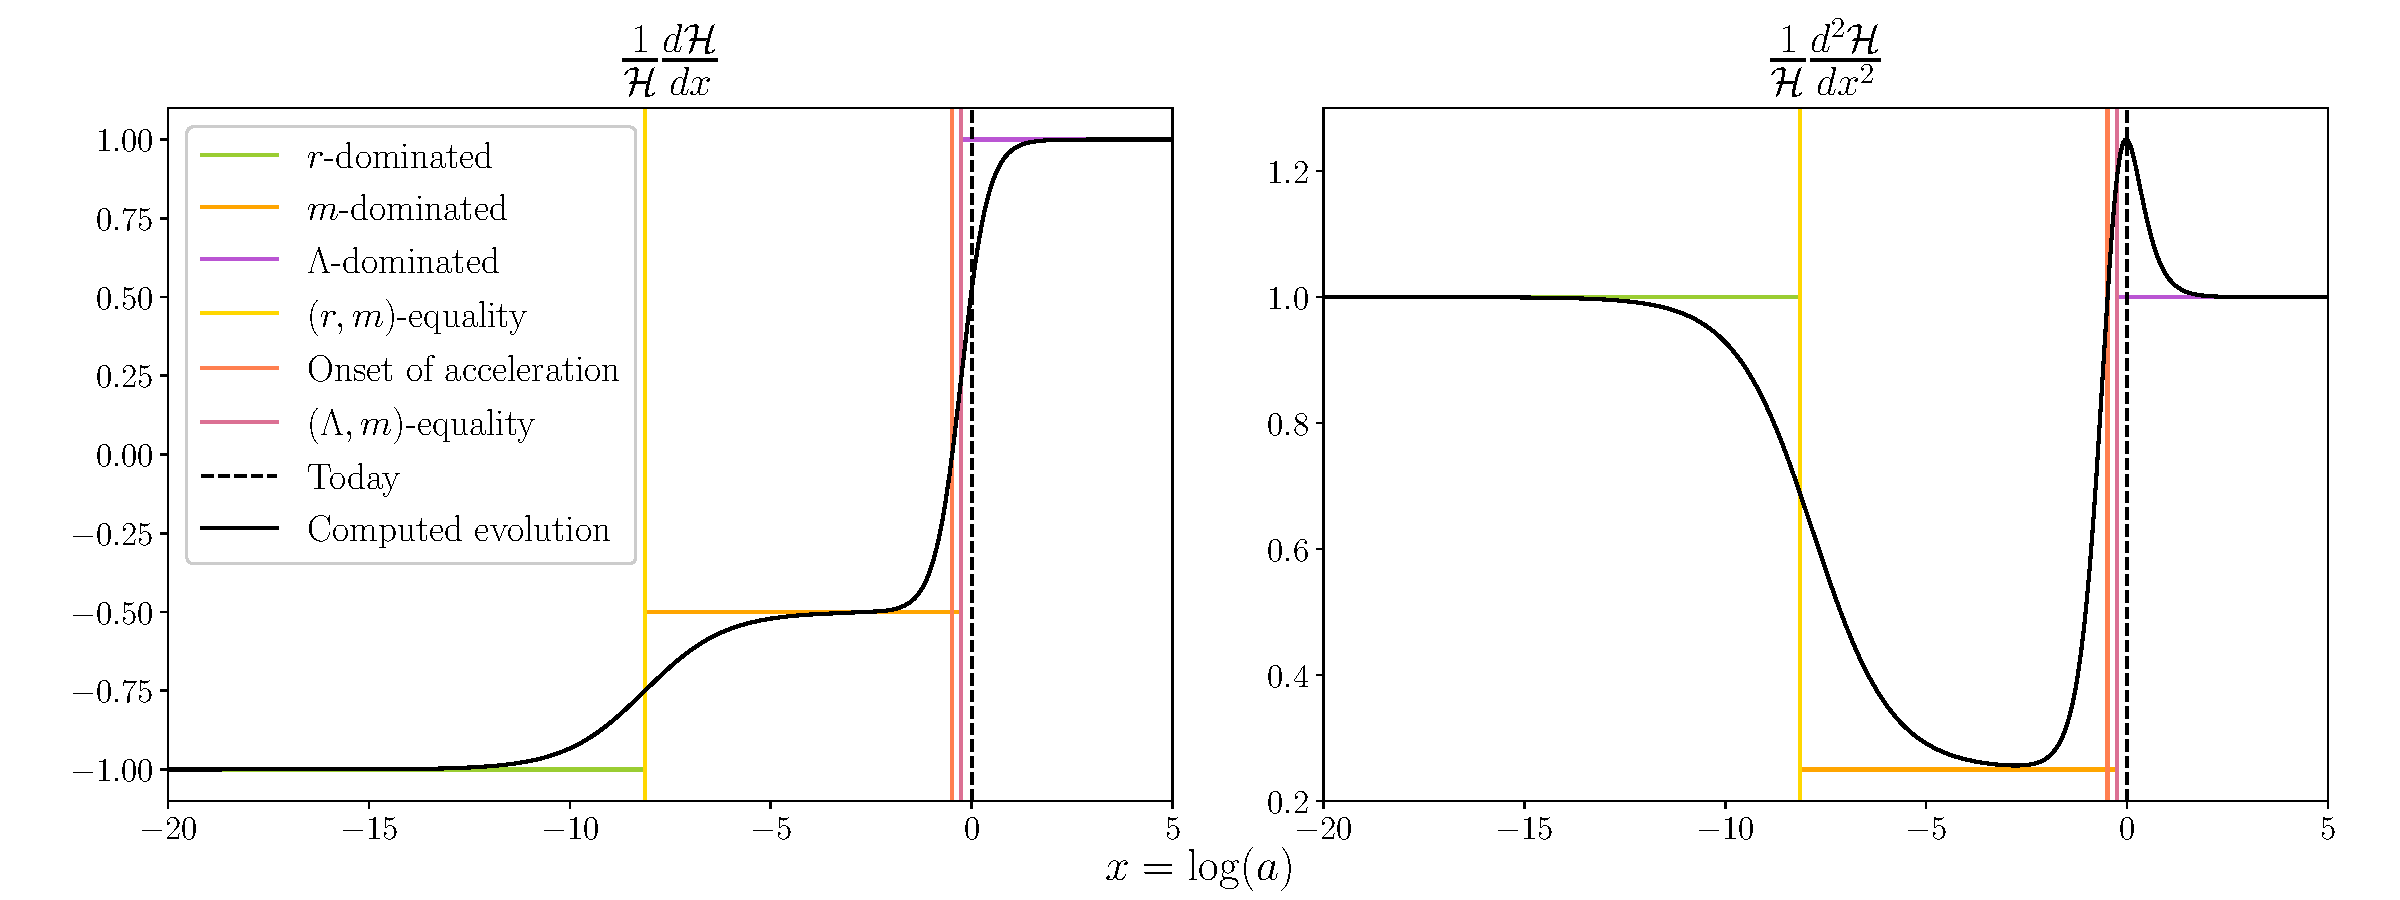
\includegraphics[width=\textwidth]{/Users/paljettrosa/Documents/GitHub/AST5220/figs/H_prime_derivatives.pdf}
    \caption{Comparison of exact evolutions (black) with approximations (dashed) for the scaled first and second derivatives of $\mathcal{H}(x)$. Agreement is good in pure radiation and matter domination but deviates near transitions due to neglected components.}\label{fig:H_prime derivatives}
\end{figure*}

A more direct comparison between the approximations and the exact evolution can be seen in figure \ref{fig:H_prime derivatives}, where I have plotted the first (left) and second (right) derivatives of $\mathcal{H}$ with respect to $x$, divided by $\mathcal{H}$ to see relative differences more easily. The dashed lines of different colors represent the same things here as well. We see good agreement in the asymptotically radiation-dominated and dark energy-dominated regimes, while in the matter-dominated epoch and around the equality times there are clear deviations, especially for the double derivative. This is reasonable, as we make rough approximations in both the beginning and the end of this era, hence the exact solution barely has time to sink to the expected value before it rises at the next transition point. 

It is interesting to see that the scaled double derivative actually increases beyond the expected value in the beginning of the dark energy-dominated era, with the peak being today. To understand this, we can look back at the expressions \eqref{eq:dHpdx} and \eqref{eq:ddHpddx}. The latter shows that the second derivative is influenced by a competition between growing and decaying terms as the Universe evolves: During the matter-dominated era, the dominant term is $\Omega_{m0} e^{-x}$, which leads to a slow decrease in $\mathcal{H}$; as $\Lambda$ begins to dominate, the exponential growth of the $2\Omega_{\Lambda 0} e^{2x}$ term starts accelerating the Universe. The transition is not instantaneous, meaning there is a period where the competing effects of matter dilution ($e^{-x}$) and dark energy growth ($e^{2x}$) cause a rapid shift in dynamics. This is visible in the sharp turn of $\mathcal{H}$ in figure \ref{fig:H_prime}, and explains the peak in the scaled second derivative before it settles into the $\Lambda$-dominated regime. \colorbox{Plum}{is this a reasonable analysis?}


\subsubsection{Time and horizon measures}
\begin{figure*}
  \centering
  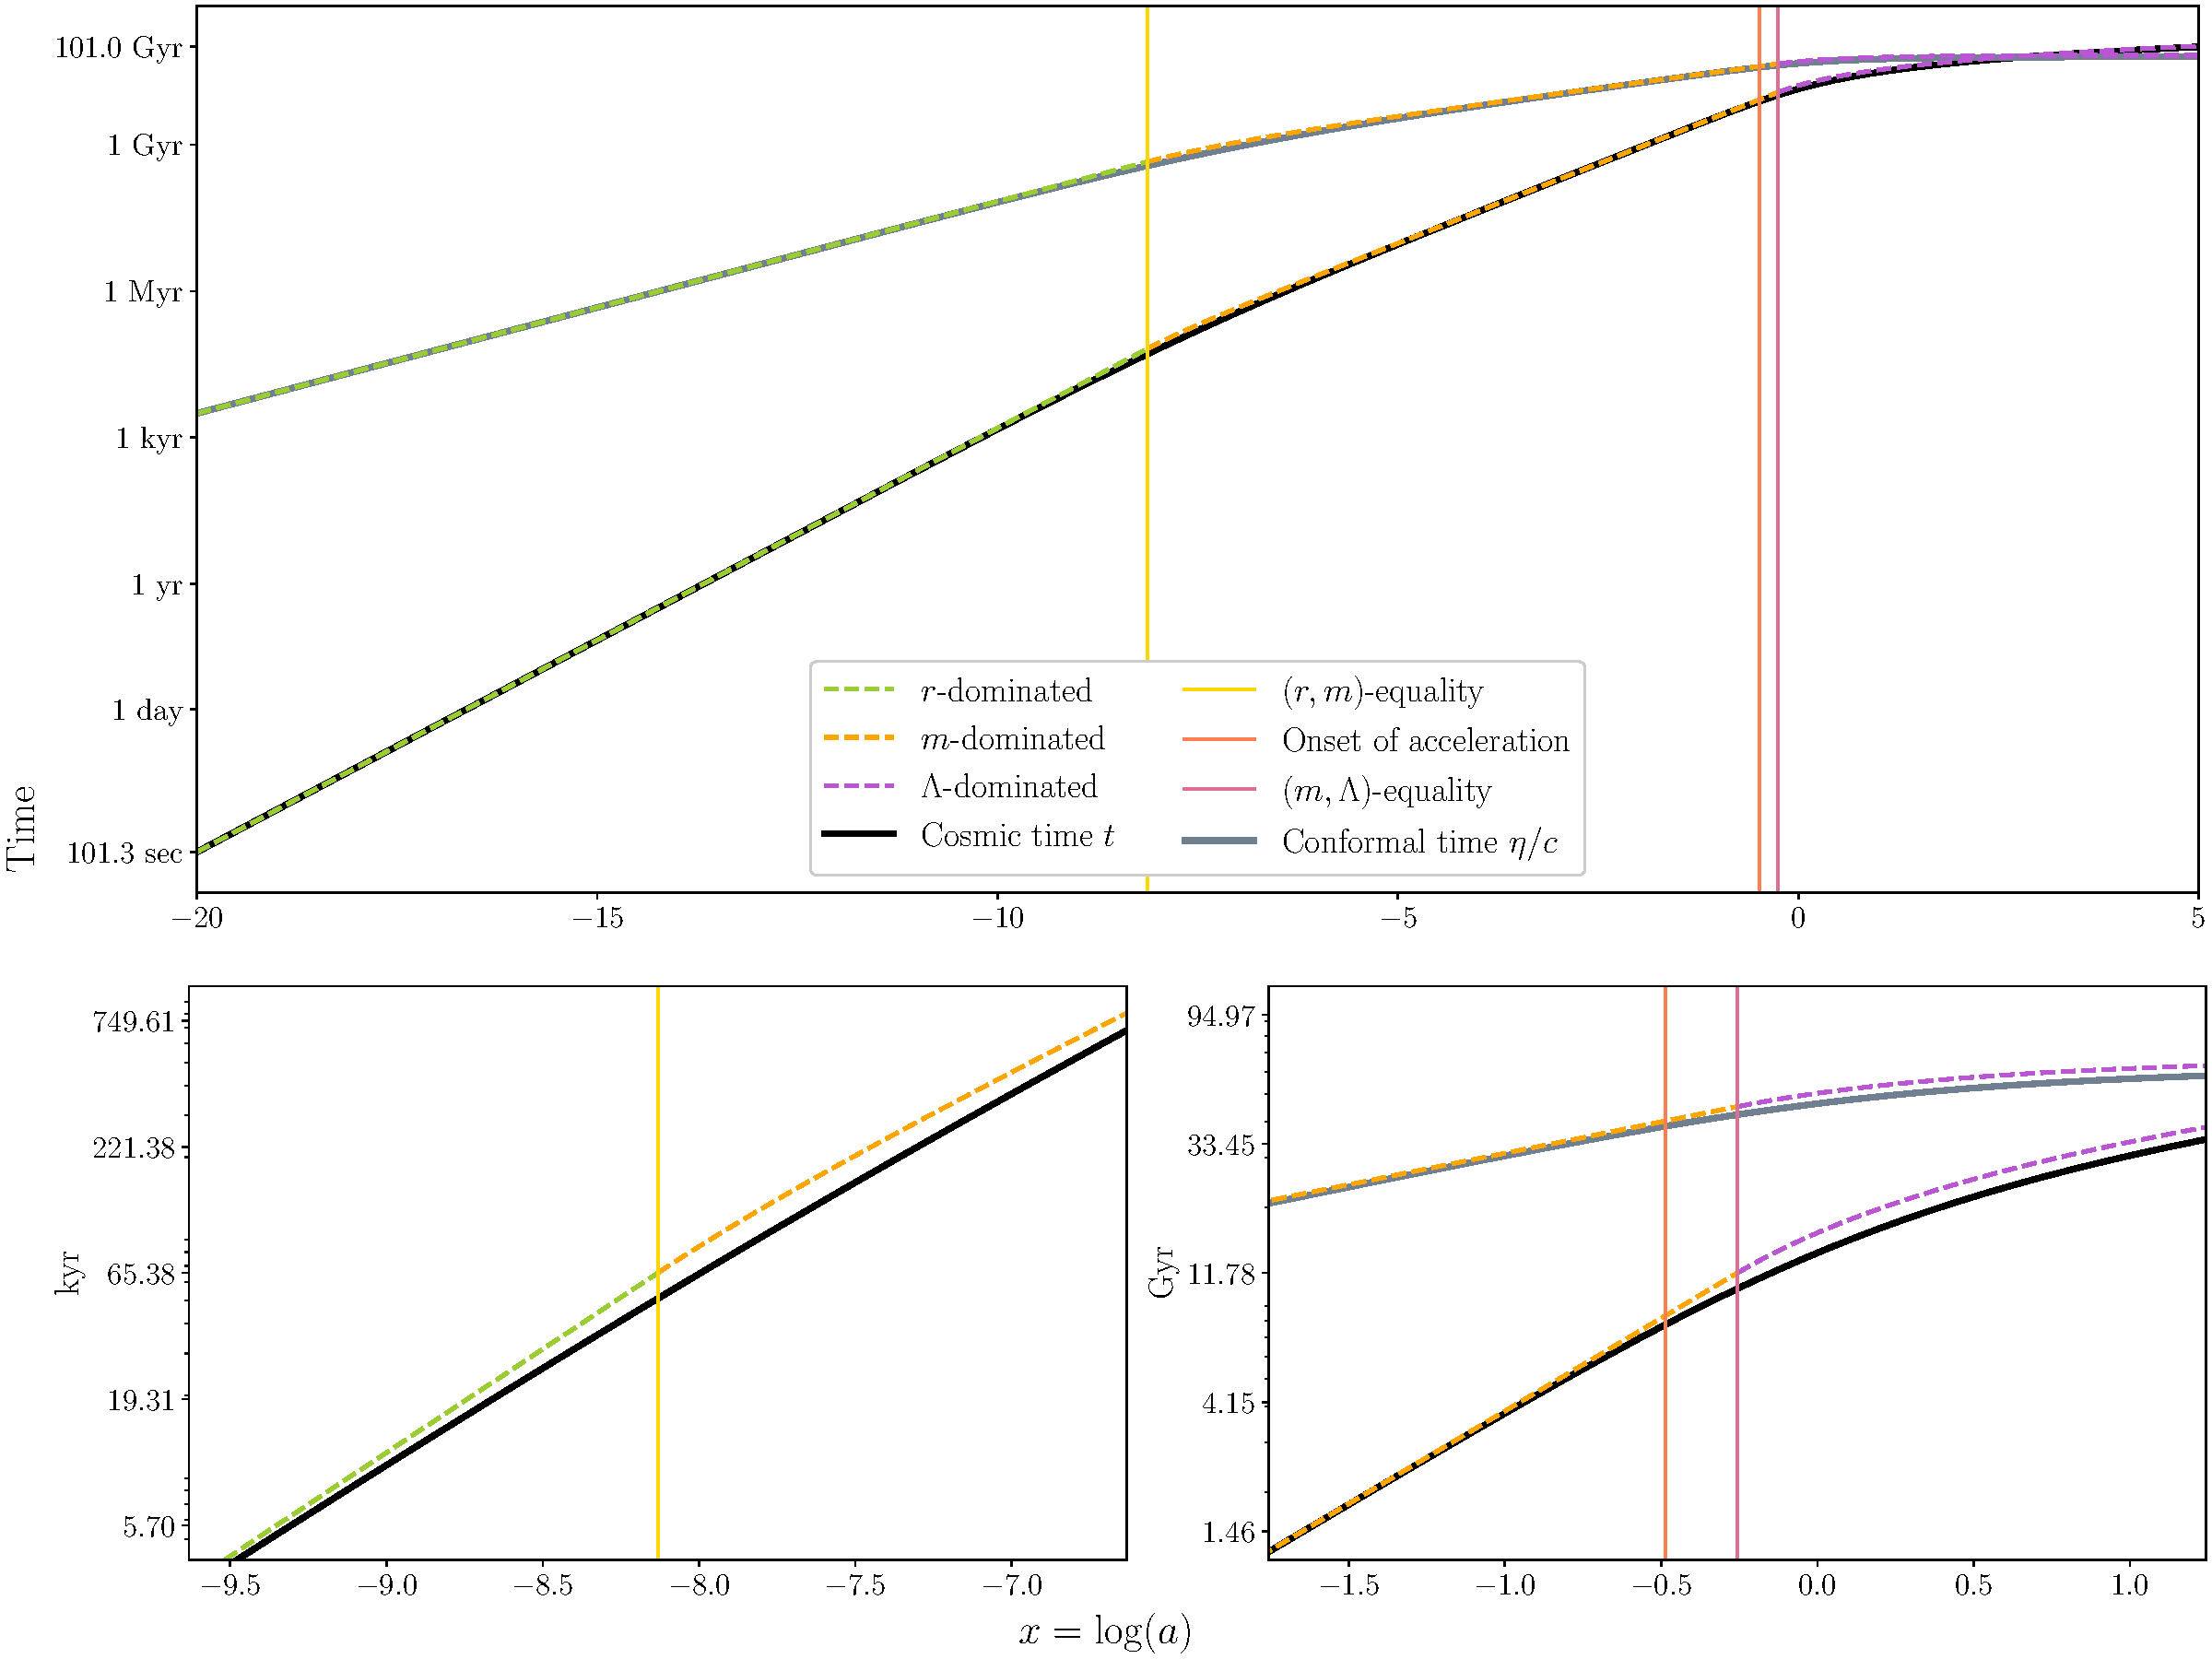
\includegraphics[width=\textwidth]{/Users/paljettrosa/Documents/GitHub/AST5220/figs/eta_and_t.pdf}
  \caption{Conformal time $\eta(x)$ (grey) and cosmic time $t(x)$ (black) compared with analytical approximations (dashed). Deviations near equality points arise due to gradual transitions between dominant energy components. This is highlighted in the bottom subplots for the cosmic time.}\label{fig:eta and t}
\end{figure*}

In figure \ref{fig:eta and t} I have plotted the numerical solutions for the conformal time $\eta/c$ (grey) and the cosmic time $t$ (black) as functions of $x$, with the approximate analytical solutions presented in section \ref{subsec: I theory} overplotted with dashed lines. The two bottom subplots, where the cosmic time is in focus, are included to easily be able to study what happens where the discrepancies between the numerical and analytical solutions are most drastic: where the Universe transitions from being dominated by one component to another. As expected, we see that the analytical approximation starts to deviate from the numerical curve as we approach $(r,m)$-equality, and eventually meets it again after. This happens also for the $(m,\Lambda)$-equality, but here the deviation actually continues to grow before it falls down again.


\begin{table*}
  \caption{Key cosmological timestamps at radiation-matter equality, the onset of acceleration, matter-dark energy equality, and present-day values. The analytical values are obtained using approximations from the theory section, while the numerical values are extracted from splines after solving the full system of equations. Discrepancies between the two highlight the limitations of the analytical approximations, especially during transition epochs.}             % title of Table
  \label{table:time stamps}      % is used to refer this table in the text
  \centering                          % used for centering table
  \begin{tabular}{| c || c | c | c | c |}        % centered columns (4 columns)
  \hline                % inserts double horizontal lines
   & Radiation-matter equality & Onset of acceleration & Matter-dark energy equality & Present day values \\    % table heading 
  \hline\hline                        % inserts single horizontal line
  \hspace{6pt}$x$\hspace{53pt} & \hspace{8.5pt}$-8.13$ & $-0.49$ & $-0.26$ & 0 \\      % inserting body of the table
  \hline 
  \hspace{6pt}$z$\hspace{53pt} & $3400.33$ & \hspace{6.5pt}$0.63$ & \hspace{7pt}$0.29$  & 0 \\
  \hline 
  \hspace{6pt}$t$ \hspace{5pt}(analytical) & \hspace{25pt}$65.38\,$kyr & \hspace{24.5pt}$8.33\,$Gyr & \hspace{19pt}$11.78\,$Gyr & \hspace{25pt}$16.30\,$Gyr \\
  \hspace{6pt}$t$ \hspace{5pt}(numerical) & \hspace{25pt}$51.06\,$kyr & \hspace{24.5pt}$7.75\,$Gyr & \hspace{19pt}$10.38\,$Gyr & \hspace{25pt}$13.86\,$Gyr \\
  \hline 
     $\eta/c$ (analytical) & \hspace{25pt}$444.75\,$Myr & \hspace{20.5pt}$40.22\,$Gyr & \hspace{19pt}$45.20\,$Gyr & \hspace{25pt}$50.36\,$Gyr \\ 
     $\eta/c$ (numerical) & \hspace{25pt}$368.44\,$Myr & \hspace{20.5pt}$38.57\,$Gyr & \hspace{19pt}$42.37\,$Gyr & \hspace{25pt}$46.32\,$Gyr \\ 
     \hline 
     \hspace{5.5pt}$\eta$ \hspace{3.5pt}(analytical) & \hspace{25pt}$136.27\,$Mpc & \hspace{20.5pt}$12.32\,$Gpc & \hspace{19pt}$13.85\,$Gpc & \hspace{25pt}$15.43\,$Gpc \\ 
     \hspace{5.5pt}$\eta$ \hspace{3.5pt}(numerical) & \hspace{25pt}$112.89\,$Mpc & \hspace{20.5pt}$11.82\,$Gpc & \hspace{19pt}$12.98\,$Gpc & \hspace{25pt}$14.19\,$Gpc \\ 
  \hline                                   %inserts single line
  \end{tabular}
  \end{table*}

In table \ref{table:time stamps} I have listed key cosmological timestamps for important transition points in the Universe's history: radiation-matter equality, the onset of acceleration, matter-dark energy equality, and present-day values. The logarithmic scale factor $x = \log a$ and redshift $z$ are listed for each event, along with analytical and numerical results for cosmic time $t$, conformal time $\eta/c$, and the comoving horizon $\eta$. We observe a discrepancy between the analytically approximated values for $t$ and $\eta$ obtained using the expressions derived in section \ref{subsec: I theory} and the corresponding numerical values, which instead were obtained by solving the full system of equations and interpolating via splines. These discrepancies are consistent with figure \ref{fig:eta and t}.

The age of the Universe is presented as $t_0=13.801\pm0.024\,\text{Gyr}$ in \citet{Planck}, an estimate based on $1\sigma$ constraints on a combination of gravitational lensing and TT (temperature), TE (temperature-E mode polarization), EE (E mode polarization) and lowE (low multipole E-mode polarization) angular power spectra measurements. This is in good agreement with the numerical result, although the value stated here is slightly larger. Nevertheless, the analytical approximation greatly overestimate it in comparison. This further validates the numerical solution around the equality times, where it deviates from the approximate evolutions and we have less to compare it to.

\subsubsection{Density parameters}
\begin{figure}
    \centering
    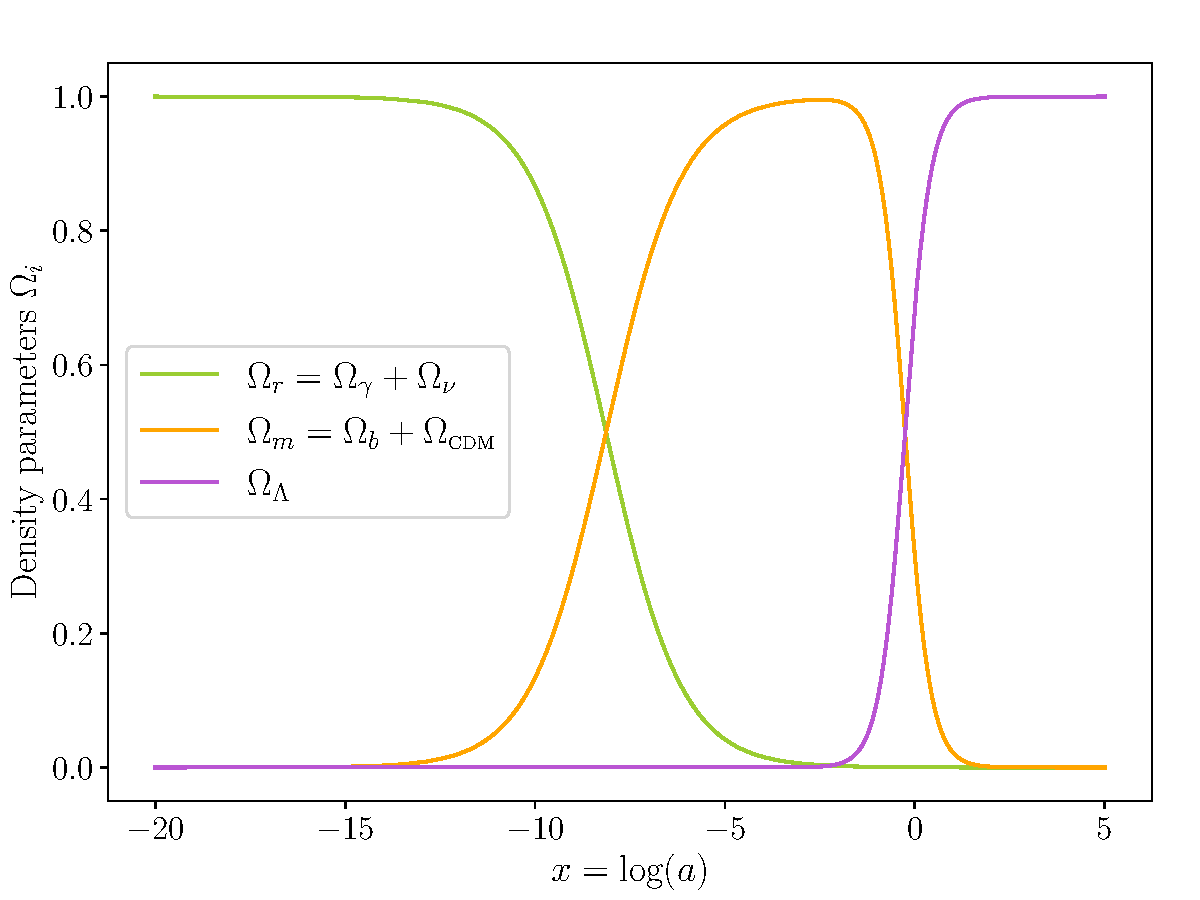
\includegraphics[width=\columnwidth]{/Users/paljettrosa/Documents/GitHub/AST5220/figs/density_parameters.pdf}
    \caption{The fractional energy densities of radiation, matter, and dark energy as functions of $x$ (solid lines). The dashed lines show the evolutions of the radiation components (photons and neutrinos) and matter components (baryons and dark matter).}\label{fig:density parameters}
\end{figure}

The evolutions of the density parameters $\Omega_i(x)$ are plotted in figure \ref{fig:density parameters}, with solid lines for $\Omega_r$, $\Omega_m$ and $\Omega_\Lambda$, and dashed lines for the individual components that make up the two first of these. The solid curves are consistent with the previous results, with the transitions between the different eras matching the observed changes in $\mathcal{H}$, $\eta$ and $t$. For example, the abrupt change in the conformal Hubble parameter at $(m,\Lambda)$-equality compared to the change at $(r,m)$-equality matches the relatively rapid takeover of $\Lambda$ as the dominating energy component, as opposed to the more gradual change from radiation to matter domination. 

\subsubsection{Supernova fitting}
\begin{table}
  \caption{Best-fit cosmological parameters obtained from supernova data, along with their mean values and standard deviations. The best-fit values correspond to the minimum $\chi^2$, while the Planck 2018 values are provided for comparison. The Hubble constant $H_0$ is given in units of km/s/Mpc.}             % title of Table
  \label{table:supernova}      % is used to refer this table in the text
  \centering                          % used for centering table
  \begin{tabular}{| c || c | c | c | c |}        % centered columns (4 columns)
  \hline                % inserts double horizontal lines
   & \hspace{5pt}$\mu_i$\hspace{5pt} & \hspace{7pt}$\sigma_i$\hspace{7pt} & min$\big(\chi^2\big)$ & Planck \\    % table heading 
  \hline\hline                     % inserts single horizontal line
  $H_0$ & 70.112 & 0.483 & 70.204 & 67 \\
  \hline
  $\Omega_{m0}$ & \hspace{5pt}0.240 & 0.086 & \hspace{5pt}0.258 & 0.317 \\
  \hline
  $\Omega_{k0}$ & \hspace{5pt}0.118 & 0.216 & \hspace{5pt}0.071 & 0 \\
  \hline
  $\Omega_{\Lambda0}$ & \hspace{5pt}0.642 & 0.133 & \hspace{5pt}0.672 & 0.682907 \\
  \hline                                   %inserts single line
  \end{tabular}
\end{table}

When running the MCMC fits, the minimum chi-squared value obtained was $\chi^2_\text{min}=29.2867$, corresponding to the parameter values listed in the third column of table \ref{table:supernova}. The means $\mu_i$ and standard deviations $\sigma_i$ (where $i$ runs over the parameters) computed for the samples within the $1\sigma$ constraints are listed as well, in addition to the Planck parameters for comparison. Interestingly, the results favor a slightly open universe, deviating from the Planck result of a flat universe. However, the standard deviation, which is about three times larger than the best-fit value, suggests that the data does not strongly constrain curvature. We also see that the Planck result for $\Omega_{m0}$ is higher than the best-fit value, though it is within the $1\sigma_m$ confidence interval. \colorbox{Plum}{correct to say this?} Nevertheless, this suggests that the supernova data prefers a lower matter density, which is consistent with the higher inferred value of $H_0$. 
% Lastly, the Planck value for $\Omega_{\Lambda0}$ is only slightly larger than the best-fit value, and it is well within $1\sigma_\Lambda$. \colorbox{Plum}{correct to say this?}.

\begin{figure}
    \centering
    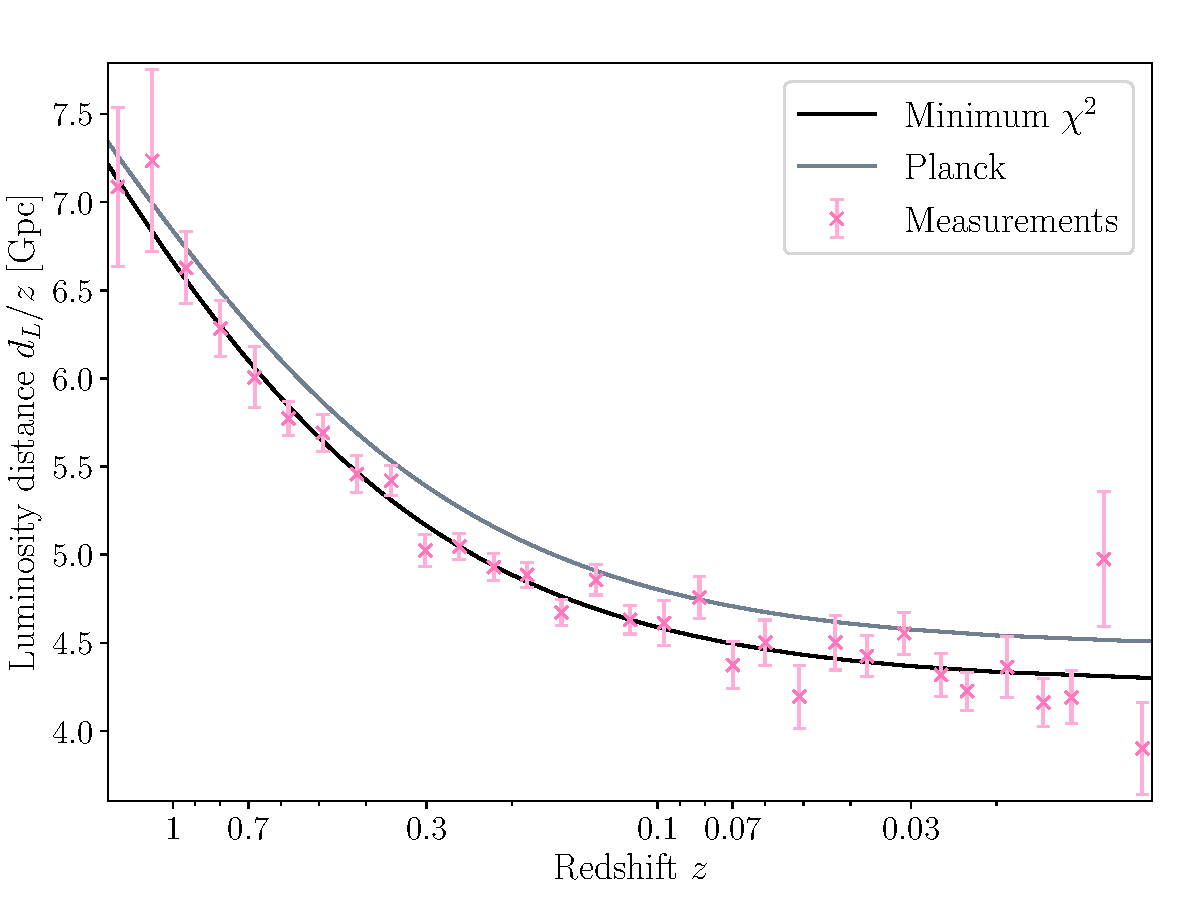
\includegraphics[width=\columnwidth]{/Users/paljettrosa/Documents/GitHub/AST5220/figs/luminosity_distance.pdf}
    \caption{Comparison of the luminosity distances $d_L^\text{obs}/z$ gathered from supernova observations (pink with errorbars) with the fiducial Planck model (grey) and the best-fit model from MCMC analysis (black).}\label{fig:luminosity distance}
\end{figure}

After obtaining the best-fit values I made a new instance of \verb|BackgroundCosmology| with these parameters and solved for this universe as well. In figure \ref{fig:luminosity distance} I have plotted the scaled luminosity distance $d_L/z$ against $z$ for this best-fit cosmology (black curve) as well as the Planck cosmology (grey curve), together with the data points $d_L^\text{obs}/z$ with scaled errorbars (pink). We see that the best-fit cosmology aligns much better with the data points than the Planck model, as it does not always lie within the supernova errorbars. The former fact is not suprising, considering that the Planck result assumes a flat universe, whereas the best-fit suggests slightly positive curvature, which alters the distance-redshift relation. The latter is more peculiar, and it highlights tensions between low-redshift and high-redshift cosmological probes. However, it should be kept in mind that measurements of supernova magnitudes can be affected by calibration uncertainties, host galaxy effects and dust extinction, potentially shifting best-fit cosmological parameters. Nevertheless, the discrepancies underscore the importance of using multiple probes and datasets to break parameter degeneracies and obtain a more complete picture of cosmic expansion.


\begin{figure}
    \centering
    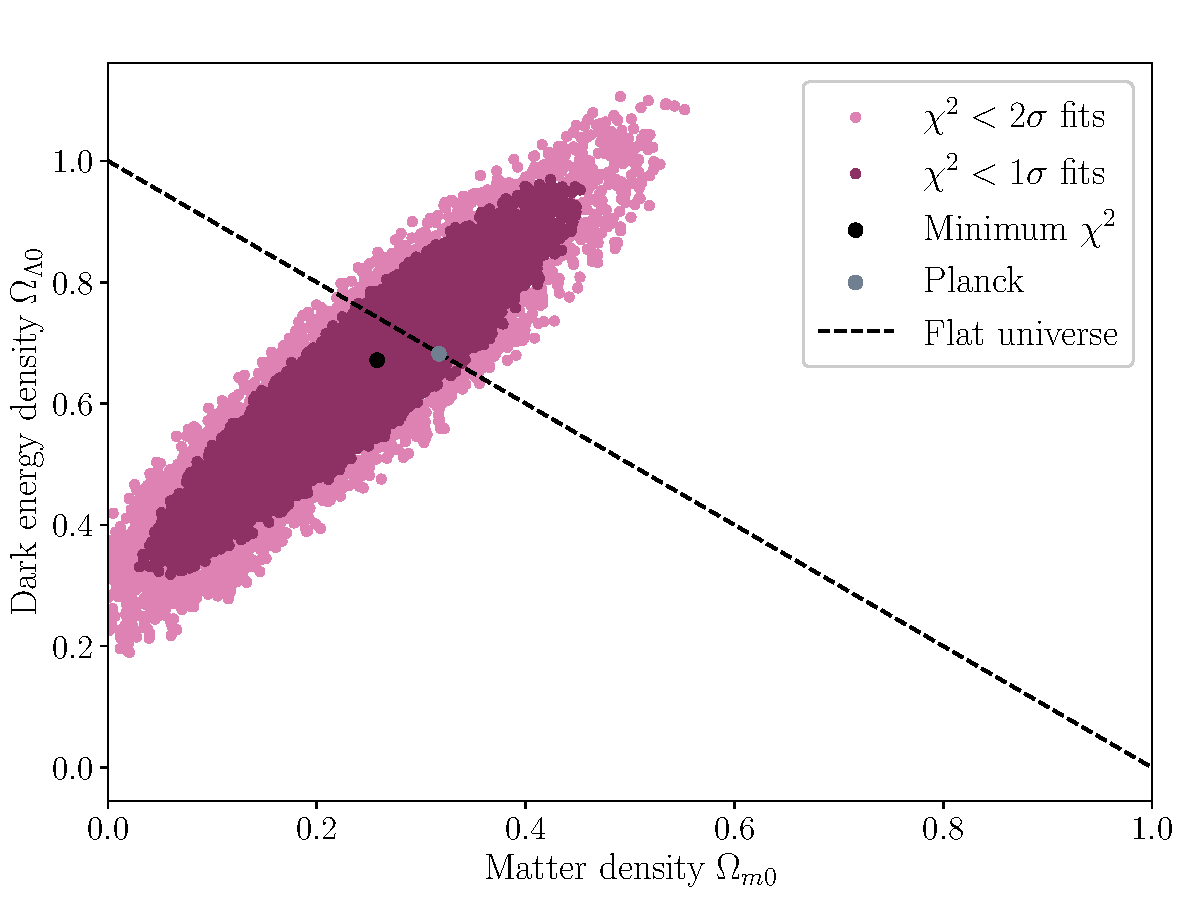
\includegraphics[width=\columnwidth]{/Users/paljettrosa/Documents/GitHub/AST5220/figs/MCMC_fits.pdf}
    \caption{Confidence contours in the $(\Omega_{m0},\Omega_{\Lambda0})$ parameter space from the supernova MCMC analysis, compared to the Planck fiducial model. The supernova constraints allow for a slightly open universe, while Planck favors flatness based on multi-probe data.}\label{fig:MCMC fits}
\end{figure}

In figure \ref{fig:MCMC fits} I have scatter plotted the accepted $(\Omega_{m0},\Omega_{\Lambda0})$ samples within the $1\sigma$ and $2\sigma$ constraints, with the black (grey) data point showing the best-fit (Planck) parameter set, and the dashed line showing the combinations that allow for a flat universe. We see clearly here that supernova-only constraints allow for slightly different cosmologies than the Planck model, with a preference for a lower matter density and small positive curvature. The Planck data includes additional information from the early universe, leading to a tighter preference for a flat universe with more mass. This discrepancy ties directly to the luminosity distance plot, confirming that these best-fit supernova parameters slightly differ from Planck's and further highlighting the importance of combining multiple datasets for robust cosmological constraints.


% When running the MCMC fits, the minimum chi-squared value obtained was $\chi^2_\text{min}=29.2867$, corresponding to the parameter values listed in the third column of table \ref{table:supernova}. The means $\mu_i$ and standard deviations $\sigma_i$ (where $i$ runs over the parameters) computed for the samples within the $1\sigma$ constraints are listed as well, in addition to the Planck parameters for comparison. We see that the best-fit value of $H_0$ based on the supernova data alone was $70.204\,$km/s/Mpc, slightly higher than the Planck result of $67\,$km/s/Mpc. This is expected, as supernova data alone tends to favor a higher $H_0$ than CMB-based analyses, a discrepancy known as the Hubble tension. We also see that the Planck result is larger than the best-fit value for $\Omega_{m0}$, though it is within $1\sigma_m$ \colorbox{Plum}{correct to say this?}. Nevertheless, this suggests that the supernova data prefers a lower matter density, which is consistent with the higher inferred value of $H_0$.

% Interestingly, the results favor a slightly open universe, deviating from the Planck result of a flat universe. However, the standard deviation, which is about three times larger than the best-fit value, suggests that the data does not strongly constrain curvature. Lastly, the Planck value for $\Omega_{\Lambda0}$ is only slightly larger than the best-fit value, and it is well within $1\sigma_\Lambda$. \colorbox{Plum}{correct to say this?}. These results highlight the differences between constraints obtained from supernova data alone versus those obtained from CMB measurements. The larger uncertainties in our fits, particularly for $\Omega_{k0}$, emphasize the need to incorporate additional cosmological probes, such as baryon acoustic oscillations (BAO) and CMB data, for tighter constraints.

\begin{figure*}
  \centering
  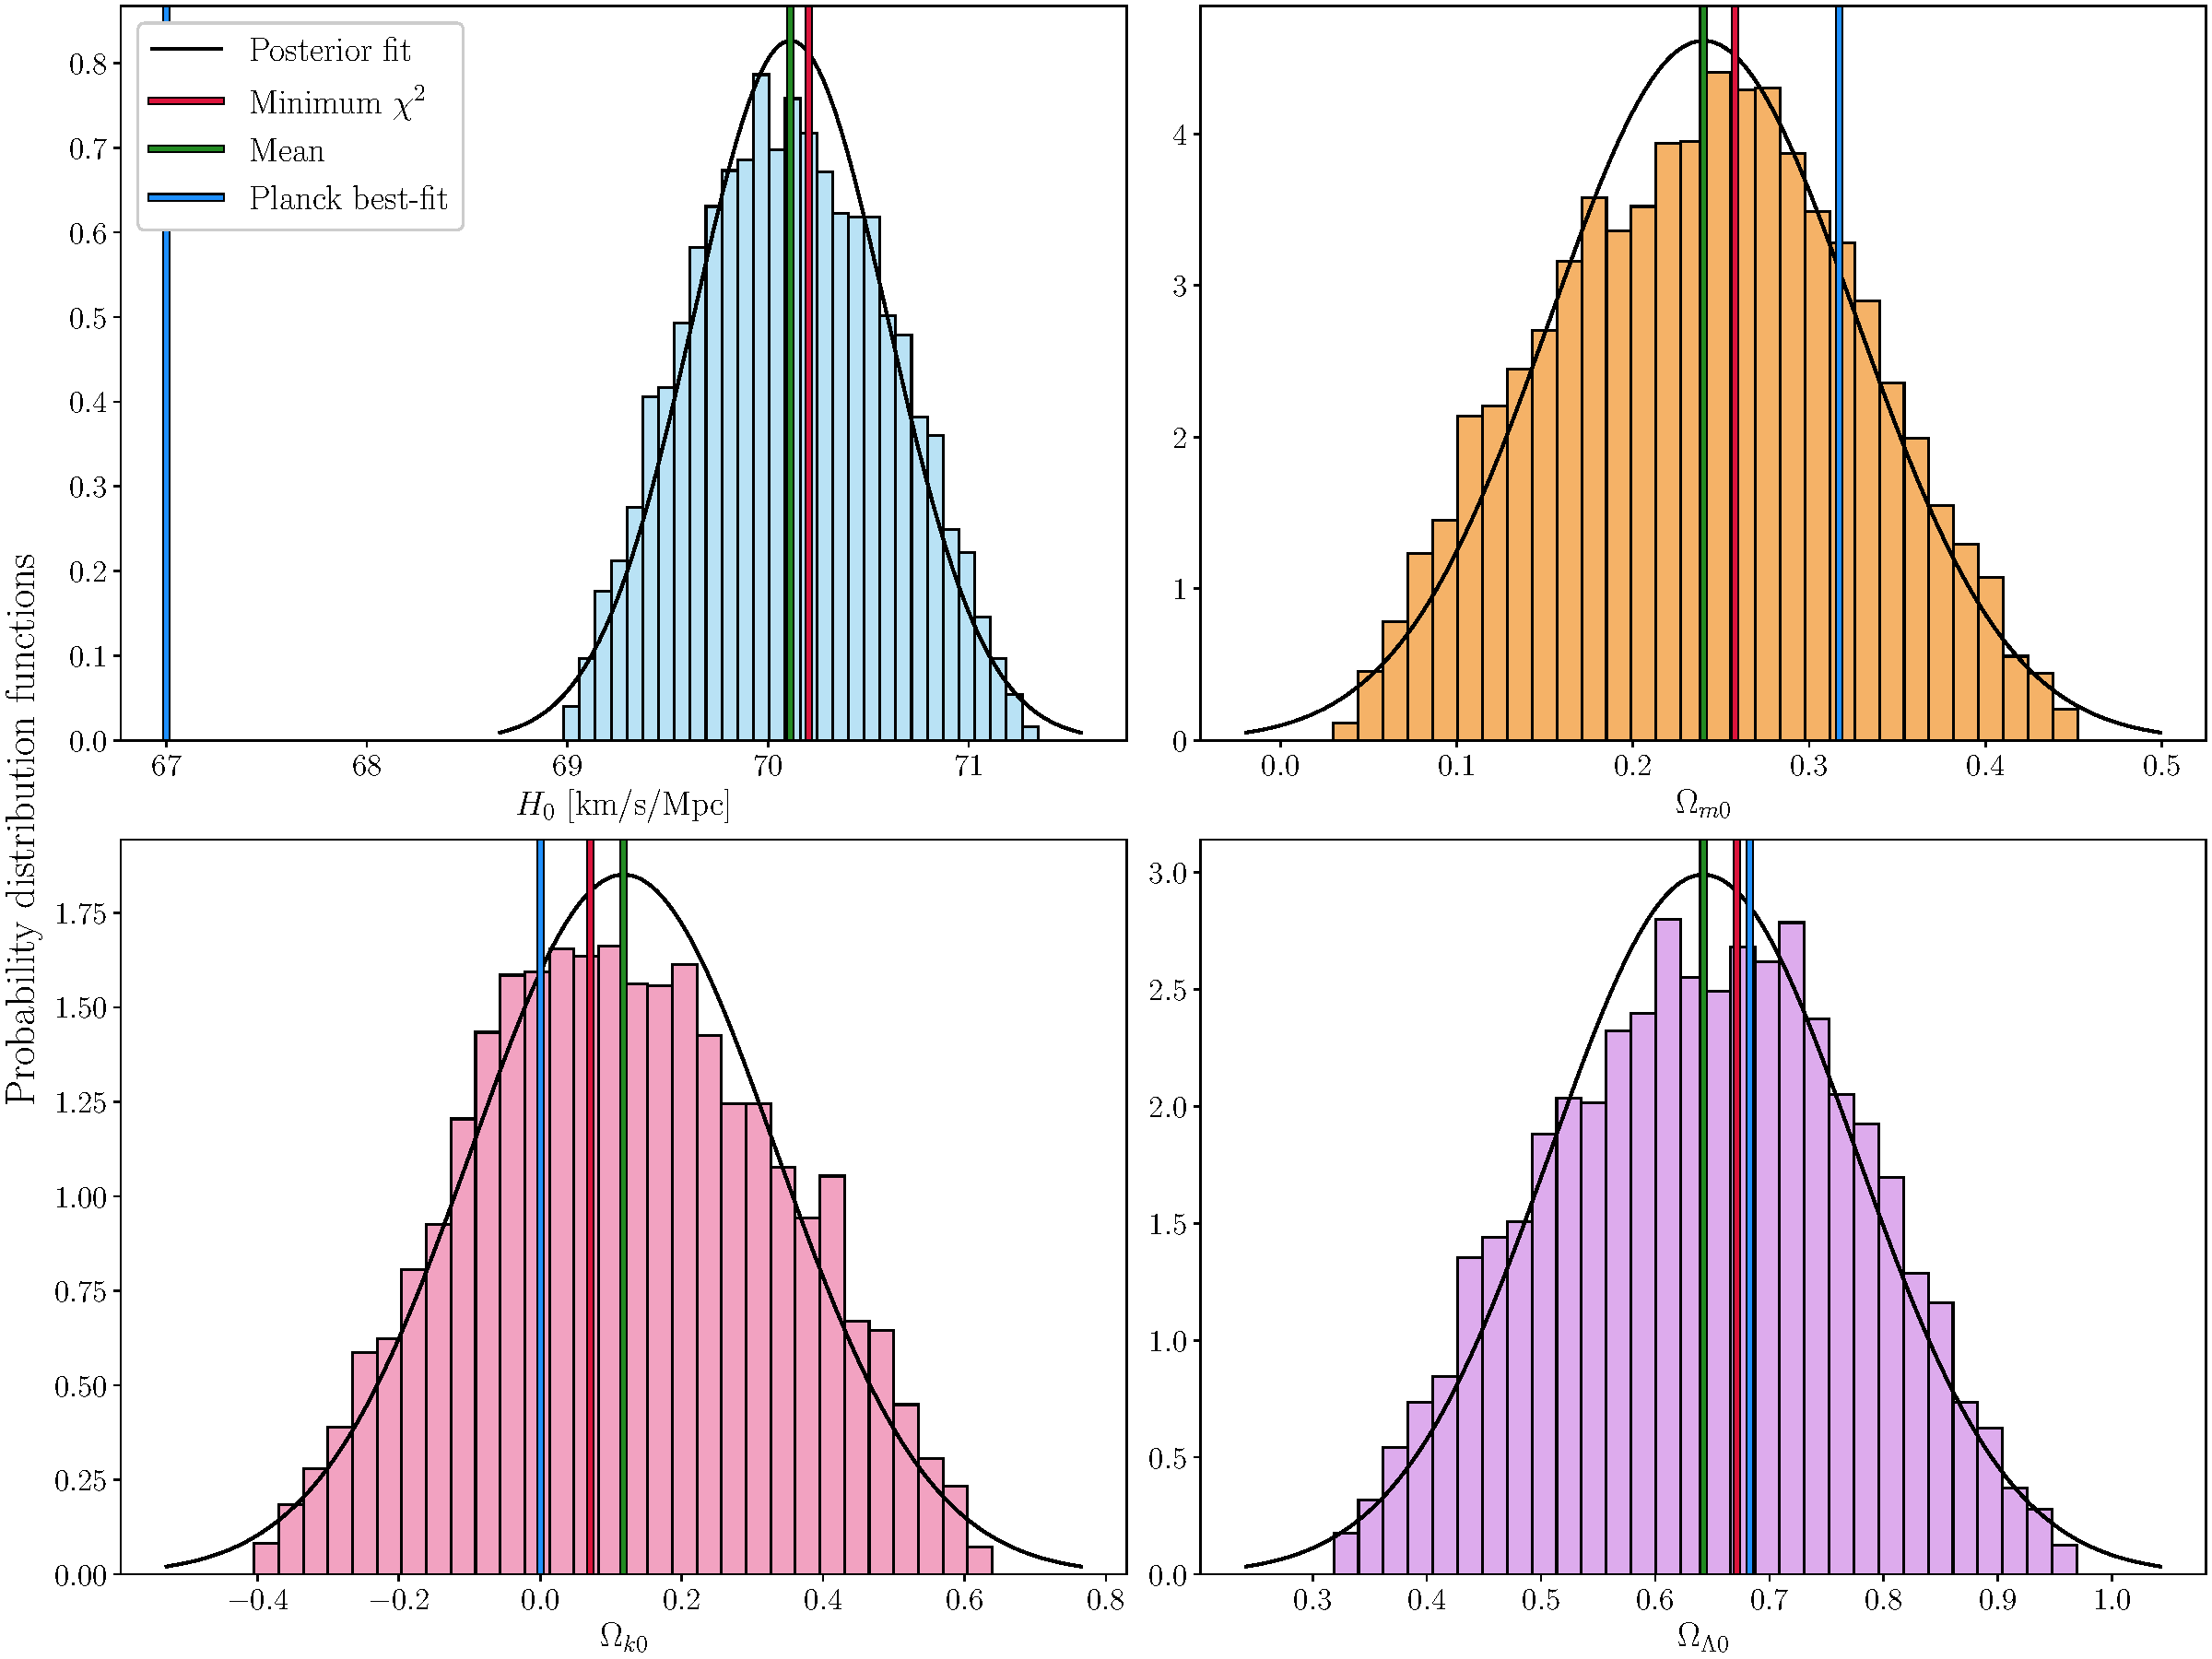
\includegraphics[width=\textwidth]{/Users/paljettrosa/Documents/GitHub/AST5220/figs/distributions.pdf}
  \caption{Histograms of the MCMC posterior distributions for the parameters $(H_0,\Omega_{m0}, \Omega_{k0}, \Omega_{\Lambda0})$, compared with Gaussian fits (solid curves) and Planck values. Deviations from Gaussianity indicate asymmetries in parameter uncertainties.}\label{fig:distributions}
\end{figure*}

Figure \ref{fig:distributions} shows normalized histograms of the samples within the 1$\sigma$ constraint, with Gaussian fits made with the $\mu_i$ and $\sigma_i$ overplotted to represent the posterior distributions. Most noticeable is how different the supernova and Planck results are for $H_0$, with the smallest accepted $1\sigma$ samples being as large as $69\,$km/s/Mpc. Planck's estimate is derived from early universe physics (CMB, BAO, and LSS), while supernova constraints come from low-redshift expansion. The discrepancy may therefore indicate new and/or unknown physics present at some eras of the expansion history, or possibly systematic errors in one or both datasets. Moreover, we see that the supernova-only constraint clearly prefers a lower matter density compared than the Planck estimate, consistent with the MCMC contour plot.

The posterior distribution suggests a preference for a slightly open universe, though with considerable uncertainty. This deviation from flatness may arise because supernovae alone do not tightly constrain curvature, as they primarily measure relative distances, not absolute spatial curvature. Moreover, we see that the histograms are not perfectly Gaussian, particularly those for $\Omega_{m0}$ and $\Omega_{k0}$. Specifically, the asymmetry with more samples in the low mass/positive curvature ends suggest a skewed uncertainty, indicating that a simple Gaussian error estimate might underestimate the possible range of accepted values. \colorbox{Plum}{does this make sense?} Alarmingly, the $H_0$ distribution appears more symmetric, indicating that supernova data alone provide a more stable estimate for the Hubble constant, which deviates the most from the Planck result.




\section{Milestone II: Recombination History}\label{sec: milestone II}
% In the previous milestone, I established a robust numerical framework for studying the background evolution of the Universe, validating my methods by comparing with analytical approximations and observational constraints. By solving for the cosmic and conformal time evolution, as well as constraining key cosmological parameters using Type Ia supernova data, we have gained insights into the expansion history and geometry of the Universe. However, a complete understanding of cosmic evolution requires accounting for the interactions between matter and radiation. The next milestone will focus on modeling the recombination history, which is essential for understanding the formation of the cosmic microwave background and the transition from an ionized to a neutral Universe.

\subsection{Theoretical framework}\label{subsec: II theory}

\subsection{Implementation details}\label{subsec: II methods}

\subsection{Results and discussions}\label{subsec: II results}



\section{Milestone III: Perturbations}\label{sec: milestone III}

\subsection{Theoretical framework}\label{subsec: III theory}

\subsection{Implementation details}\label{subsec: III methods}

\subsection{Results and discussions}\label{subsec: III results}



\section{Milestone IV: Power Spectra}\label{sec: milestone IV}

\subsection{Theoretical framework}\label{subsec: IV theory}

\subsection{Implementation details}\label{subsec: IV methods}

\subsection{Results and discussions}\label{subsec: IV results}


\section{Conclusions}\label{sec: conclusions}

\bibliographystyle{aa} % style aa.bst
\bibliography{references} % your references Yourfile.bib


\end{document}